% Fragmento reutilizable: se incorpora desde un entorno figure con \input.
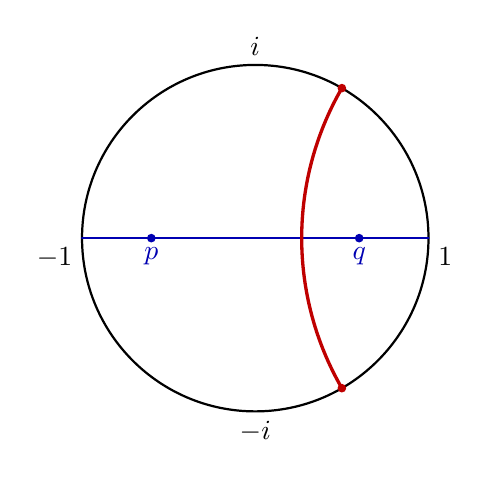
\begin{tikzpicture}[scale=2.2,line cap=round]
  \draw[thick] (0,0) circle (1cm);
  \draw[blue!70!black,thick] (-1,0) -- (1,0);
  % Arco de la circunferencia de centro (2,0) y radio sqrt(3): ortogonal al borde.
  \draw[red!75!black,very thick]
    (0.5,0.8660254) arc[start angle=150,end angle=210,radius=1.7320508cm];
  \fill[blue!70!black] (-0.6,0) circle (0.025) node[below] {$p$};
  \fill[blue!70!black] (0.6,0) circle (0.025) node[below] {$q$};
  \fill[red!75!black] (0.5,0.8660254) circle (0.025);
  \fill[red!75!black] (0.5,-0.8660254) circle (0.025);
  \node[below left] at (-1,0) {$-1$};
  \node[below right] at (1,0) {$1$};
  \node[above] at (0,1) {$i$};
  \node[below] at (0,-1) {$-i$};
\end{tikzpicture}
